The thermal model has been built as described in Section \ref{subsec:thermaltool} according to the method explained by Smith et al \cite{Smith2011}. Before the model can be used for the design it has to undergo the verification and validation process. In the first part the verification is done by comparing the analytical and numerical solutions of a copper block. In the second part two papers by Del Corso et al are used to validate the developed model with experimental data \cite{Corso2009,Corso2011}. The last part will explain the differences that were found in the verification and validation.

\subsubsection{Verification of the model using a solid copper block}
For the verification of the thermal model the analytical solution (Equation \eqref{eq:thermver}) provided by both Smith and Holman is used \cite{Smith2011,Holman2002}. Here $\gls{sym:T}_1$ is the wall temperature at $\gls{sym:t}=0$ and $\gls{sym:T}_2$ the temperature at a certain $\gls{sym:t}$ and $\gls{sym:x}$.
\begin{equation}
\gls{sym:T}_2-\gls{sym:T}_1 = \frac{2q\sqrt{\gls{sym:alphat}\gls{sym:t}/\pi}}{\gls{sym:k}\gls{sym:A}}\exp\left(\frac{-\gls{sym:x}^2}{4\gls{sym:alphat}\gls{sym:t}}\right)-\frac{q\gls{sym:x}}{\gls{sym:k}\gls{sym:A}}\left(1-erf\frac{\gls{sym:x}}{2\sqrt{\gls{sym:alphat}\gls{sym:t}}}\right)
\label{eq:thermver}
\end{equation}
Figure \ref{fig:valcop} shows a semi-infinite 0.5 $\left[m\right]$ thick copper block subjected to a constant heat flux of 30 $\left[W\cdot cm^{-2}\right]$. The block initially has a uniform temperature of 20 $\left[^{\circ}C\right]$. The error at the surface ($x = 0.00 \left[m\right]$), in the middle ($x = 0.25 \left[m\right]$) and at the back ($x = 0.50 \left[m\right]$) between the analytical and numerical solution are 1.55 \%, 4.32 \% and 15.92 \% respectively.

\begin{figure}[H]
	\centering
	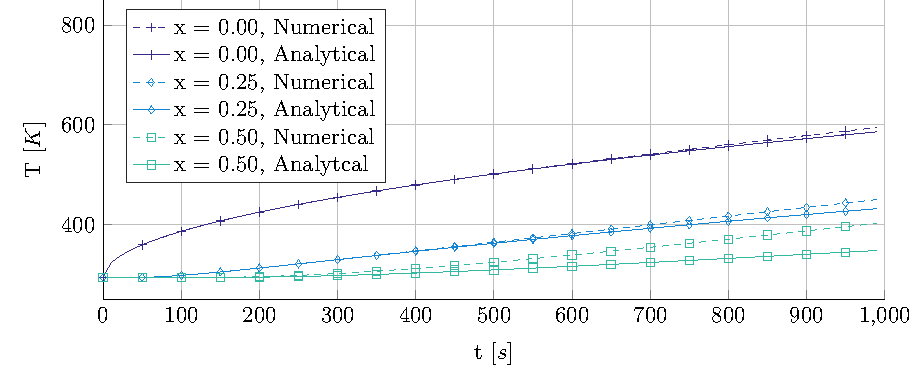
\includegraphics{Figure/Thermal/valcop.pdf}
	\caption[Comparison of analytical and numerical solution using a copper block]{Comparison of analytical and numerical solution by applying a constant heat flux for 1000 $\left[s\right]$ on a copper block with a 0.5 $\left[m\right]$ thickness.}
	\label{fig:valcop}
\end{figure}

\subsubsection{Validation against experimental data}
As mentioned earlier two papers by Del Corso provide the experimental data \cite{Corso2009,Corso2011}. Four lay-ups have been tested


\subsubsection{Conclusions after the verification and validation procedure}
The verification showed that the numerical solution starts to diverge as the error increases with time and depth. It is expected that this is a result of rounding errors that get multiplied every timestep in the discretisation scheme. The reason for this is that refining the mesh produces the same errors. There are two reasons why this is not a significant problem for the design problem. The first is that the \gls{tps} shall be a hunderd times thinner. The second is that the length of the aerocapture and entry phases are approximately 400 $\left[s\right]$, which is lower than the 1000 $\left[s\right]$ in the verification. 
 
